\chapter{Methodology Chapter}

\section{Appropriateness of the Research Design}
The following project was based on both a quantitative and qualitative approach to research techniques. Together with the amount of investigating completed collectively with this project before it had begun and throughout the developer received many high words of praise for an application of this type throughout the small and large suburbs of the Dublin area.

\section{Pilot Study of Proposed Project}
A pilot study of the application was first introduced to friends and family to get a sense of feel for if the application would be a good idea and to see if this is something that the people of Dublin would want to see coming to their mobile phones. Soon after getting a great response from family the developer chooses to produce a survey based on the people of Lucan. Based on the application and what if any specifications they would like to see. The developer received a response of over 150 people completing the survey on survey monkey. The application was indeed a certain choice for the developer to go ahead. Through wire-framing each screen that would be used throughout the application the developer had gotten an overall feel for what the end product should be.

\section{Ethical Considerations}
Each part of the project that has been carried through is deemed to be the developer's work unless stated otherwise. Other factors may contribute to the writing of this formal document and the project as a whole. Information that has to be gathered for the project as follows will be referenced appropriately. Such as that the monuments within the application itself will not be information that the developer has written but information that has been gathered from a third party. Such as an internet source which will be verified.

\section{Validity}
The data sourced for the project is to the developer's knowledge correct. Multiple sources have been read through and verified such data that is being used. Articles such as journals and other particles of information were referenced throughout to the original authors that the information was taken from or sourced.
\section{InforMe@Dublin Survey Results}
Regarding the following chapter which discussed the methodologies of why the developer chose to develop an Android application for the intended use on patrons learning about historical monuments in their area's. The results are as follows. The following survey was completed using survey monkey.

\begin{figure}[!tbp]
    \centering
    \begin{minipage}[b]{0.4\textwidth}
        \includegraphics[width=250pt]{Survey1}\\
        \caption{History Survey} 
        \label{Figure: History Survey}
    \end{minipage}
    \hfill
    \begin{minipage}[b]{0.4\textwidth}
        \includegraphics[width=250pt]{Survey2}\\
        \caption{History Survey} 
        \label{Figure: History Survey}
    \end{minipage}
\end{figure}

\begin{figure}[!tbp]
    \centering
    \begin{minipage}[b]{0.4\textwidth}
        \includegraphics[width=250pt]{Survey3}\\
        \caption{History Survey} 
        \label{Figure: History Survey}
    \end{minipage}
    \hfill
    \begin{minipage}[b]{0.4\textwidth}
            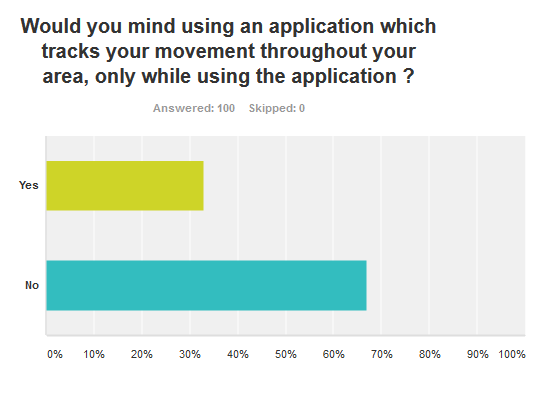
\includegraphics[width=250pt]{Survey4}\\
            \caption{History Survey} 
            \label{Figure: History Survey}
    \end{minipage}
\end{figure}
\newpage
\section{Summary}
The following chapter of which, concluded the research that has gone into choosing such a project in coherence with the BSc(Honours) Degree programme in the Institute of Technology Blanchardstown. The following was to see if the application that the developer had invented was deemed appropriate and needed in the area of Dublin. With the facts stated and nothing of the sort available online from other countries or in fact Ireland. The projects seemed plausible if the developer could, in fact, produce something of the application in mind.


